\documentclass[12pt, notitlepage]{article}   	% use "amsart" instead of "article" for AMSLaTeX format
\usepackage{geometry}                		% See geometry.pdf to learn the layout options. There are lots.
\geometry{a4paper}                   		% ... or a4paper or a5paper or ... 
%\geometry{landscape}                		% Activate for rotated page geometry
\usepackage[parfill]{parskip}    		% Activate to begin paragraphs with an empty line rather than an indent
\usepackage{graphicx}				% Use pdf, png, jpg, or eps§ with pdflatex; use eps in DVI mode
								% TeX will automatically convert eps --> pdf in pdflatex

\usepackage{hyperref}

%Use for images
\usepackage{graphicx}
\graphicspath{ {./images/} }

%SetFonts

\usepackage[T1]{fontenc}
\usepackage[utf8]{inputenc}

\usepackage{tgbonum}

%SetFonts

\title{
	\textbf{
		Mini-Quiz 1
	} \\
	\large BIOL 4301/6301 \\
	\large August 31, 2023 \\
}

\date{\vspace{-5ex}}

\def\wl{\par \vspace{\baselineskip}}

\begin{document}

{\fontfamily{phv}\selectfont %select helvetica (code = phv)

\large{Name:}

{\let\newpage\relax\maketitle}



\section{\small{What is ecosystem ecology and what makes it an important field of ecology?}}

\wl
\wl
\wl
\wl
\wl
\wl
\wl

\section{\small{In his description of the state factors controlling ecosystems and their processes,
Jenny did not include humans. How should this framework be modified based on what you've read from the Chapin book
and Vitousek paper?}}

\newpage

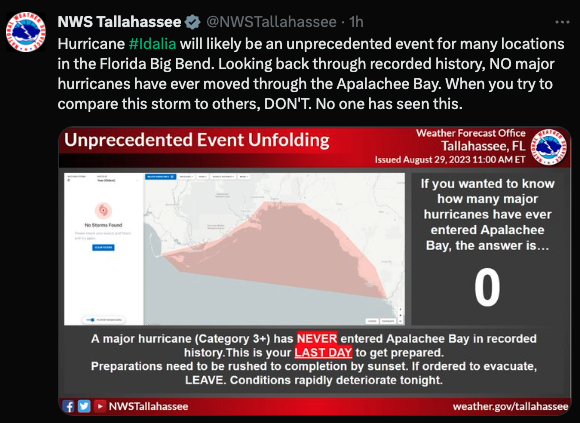
\includegraphics[scale = 0.5]{idalia_tweet}

\section{\small{The tweet (X?) above indicates that Hurricane Idalia
will impact a region in Florida (Apalachee Bay) that has never experienced a major hurricane.
Create a systems diagram to explain how Hurricane Idalia
will influence ecosystem services in the Apalachee Bay. Denote any amplifying or
stabilizing feedbacks in your diagram.}}

} %end font selection

\end{document}